\chapter{State of the Art} \label{sec:cap2}

\section{Introduction to Nuclear Fusion}

Nuclear fusion is the process in which two light atomic nuclei combine to form a heavier nucleus, releasing a substantial amount of energy. This is the same reaction that powers the Sun and other stars, making it a potential source of clean, virtually limitless energy for humanity.

The primary fuels for fusion are hydrogen isotopes such as deuterium and tritium. Their fusion produces helium and a high-energy neutron, releasing energy mainly as the kinetic energy of the neutron and, to a lesser extent, electromagnetic radiation.

Achieving controlled fusion on Earth requires overcoming the electrostatic repulsion between positively charged nuclei, which demands extremely high temperatures (on the order of tens of millions of kelvin) and sufficient pressure. These conditions can be achieved through magnetic confinement — in devices known as tokamaks — or through inertial confinement using high-power lasers.


\section{Nuclear Fusion on \acs{ITER} and \acs{JET}}

The \ac{ITER} project is an international collaboration designed to demonstrate the feasibility of nuclear fusion as a large-scale, carbon-free energy source. Under construction in Cadarache, France, ITER involves 35 countries, including members of the European Union, the United States, China, India, Japan, Russia, and South Korea. It will house the world's largest tokamak, using magnetic confinement to heat plasma to fusion conditions.\ \ac{ITER} is designed to produce ten times more fusion power than the power used to heat the plasma, representing a major step toward commercial fusion energy.

The \ac{JET} was, until December 2023, the largest operational tokamak in the world. Located in Culham, UK, it played a key role in advancing fusion research, testing plasma scenarios, and validating technologies for \ac{ITER} and future reactors. Following its final deuterium-tritium experiments, JET ceased plasma operations, and the largest operational tokamak is now JT-60SA in Japan \autocite{JT60SACertifiedWorlds2024,FusionenergyQuestMakes2024}.

The \ac{CIEMAT} is Spain's representative in \ac{EURATOM}'s fusion program, which includes participation in \ac{JET} and \ac{ITER}. For this project, \ac{CIEMAT} has provided experimental data from \ac{JET}, consisting of recorded plasma discharges.

\section{Discharges and Disruptions}

A \textit{Discharge} is a plasma operation in the tokamak, where the plasma is created and maintained for a certain period. Each discharge is characterized by various parameters, such as plasma current, inductance, density, radiated power or input power. When these parameters deviate from their expected values, it can indicate potential issues or anomalies in the reactor's operation.

A \textit{Disruption} is an event that occurs when the plasma becomes unstable and loses confinement, leading to a rapid cooling of the plasma (\textit{termal quench}) followed by a rapid loss of plasma current (\textit{current quench}). For this project, discharges are classified as either disruptive or non-disruptive.

A \textit{Campaign} is a set of discharges that are analyzed together. For this project, there are three campaigns available, each containing a different number of discharges. The available data for the project is summarized in \autoref{tab:campaigns}. This data is collected from the \ac{JET} tokamak and stored in text files for later analysis.

\begin{table}[htbp]
    \centering
    \caption{Available data for the project}
    \begin{tabular}{
        l
        S[table-format=3]  % Number of discharges
        S[table-format=2]  % Disruptive
        S[table-format=3]  % Non Disruptive
        S[table-format=1.2]@{\,}  % Rate
    }
    \toprule
    \textbf{Campaign} & \textbf{Discharges} & \textbf{Disruptive} & \textbf{Non--Disruptive} & \textbf{Disruption Rate} \\
    \midrule
    C23 & 522 & 32 & 490 & 6.13 \ \% \\
    C24 & 388 & 26 & 362 & 6.70 \ \% \\
    C25 & 611 & 41 & 570 & 6.71 \ \% \\
    \bottomrule
    \end{tabular}
    \label{tab:campaigns}
\end{table}

A visual representation of the plasma current on several discharges is shown in \autoref{fig:plasma-current}. This figure illustrates the singular bathtub shape of non-disruptive discharges, whereas disruptive discharges show a more erratic pattern.

\begin{figure}[H]
    \centering
    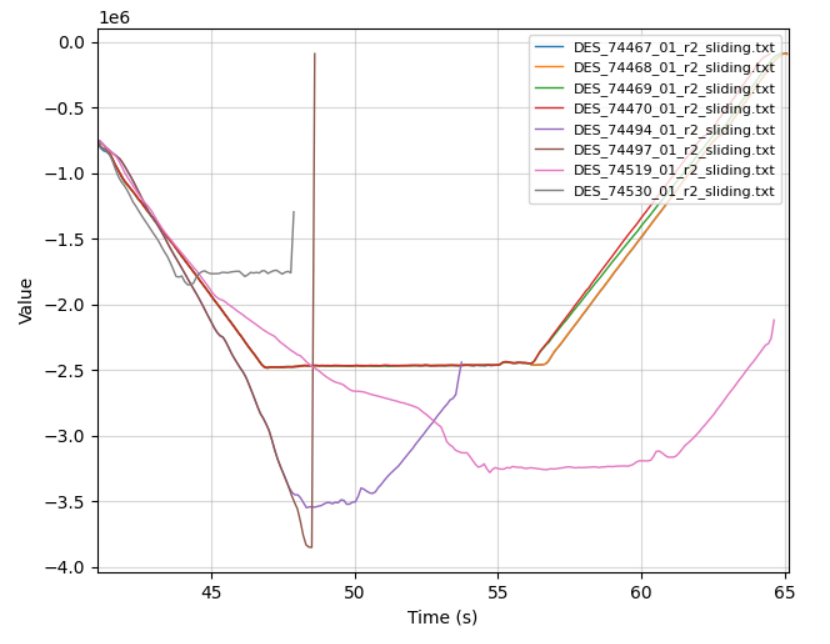
\includegraphics[width=0.8\textwidth]{plasma-current.png}
    \caption{Plasma current on disruptive and non-disruptive discharges}
    \label{fig:plasma-current}
\end{figure}

\section{Anomaly Detection in Nuclear Fusion}

Anomaly detection in nuclear fusion is crucial for ensuring the safe and efficient operation of reactors like \ac{ITER}. The complexity of the plasma behavior and the multitude of parameters involved make it challenging to monitor and control the system effectively. Anomalies can lead to disruptions, which can damage the reactor components and affect the overall performance.

To address this challenge, various machine learning techniques have been applied to analyze the data generated during discharges. These techniques aim to identify patterns and deviations in the data that may indicate potential anomalies. An early detection of these anomalies is essential to prevent disruptions and ensure the stability of the plasma, using gas injection to stop the nuclear fusion reaction before it causes damage to the reactor.

There are two main approaches to anomaly detection in nuclear fusion: neural-network-based models and physical models. Neural networks are trained on historical data to learn the patterns of normal operation, and then used to detect anomalies in real-time data. Physical models, on the other hand, are based on the physics of the plasma and are used to predict the behavior of the plasma under different conditions.

Neural networks have shown promising results in detecting anomalies, but some studies have raised concerns about their reliability and generalization capabilities.\ \textcite[p.~S188]{henderChapter3MHD2007} identify intrinsic limitations of neural-network disruption predictors—most notably, intrinsically poor extrapolation when entering new or expanded operating regimes—and argue that methods intended for a next-step device must rely on a high-quality, well-normalized, multi-machine, dimensionless database. In the same vein, \textcite[p.~2]{murariControlOrientedStrategy2024} report that device-specific ML predictors are typically limited to their tokamak of origin and that their extrapolation to larger, future devices (e.g., \ac{ITER}) is doubtful, owing to differences in scale (stored energy, $I_p$, $\beta_N$), materials and wall conditions, actuator authority, and disruption phenomenology. Taken together, these results imply that models trained solely on historical data from present machines cannot be trusted \emph{a priori} on ITER without cross-machine validation, physics-informed inductive biases, domain adaptation to covariate/concept shift, and calibrated uncertainty quantification.



\subsection{Introduction to \acs{APODIS}}

\ac{CIEMAT} uses the \ac{APODIS} algorithm, which is based on a \ac{SVM} model trained on historical discharge data.\ \ac{SVM} is a machine learning algorithm whose goal is to find the optimal hyperplane that separates the data into different classes \autocite{6524743}. Further explanation of \ac{SVM} is provided in \autoref{sec:svm}.

The model is designed to classify discharges as normal or anomalous based on the input parameters. The training process involves using labeled data, where each discharge is categorized as either normal or anomalous.

The \ac{APODIS} algorithm uses the signals listed in \autoref{tab:apodis-signals}.

\begin{table}[htbp]
  \centering
  \caption{List of signals analyzed in the \ac{APODIS} algorithm}
  \label{tab:apodis-signals}
  \begin{tabular}{@{}l c@{}}
    \toprule
    \textbf{Signal Name} & \textbf{Units} \\
    \midrule
    (1) Plasma Current                             & \si{A} \ \ \  \\
    (2) Mode Lock Amplitude                        & \si{T} \ \ \  \\
    (3) Plasma internal inductance                 &             \\ % adimensional
    (4) Plasma density                             & \si{\per\cubic\metre} \\
    (5) Stored diamagnetic energy time derivative  & \si{W} \ \ \  \\
    (6) Radiated Power                             & \si{W} \ \ \  \\
    (7) Total Input power                          & \si{W} \ \ \  \\
    \bottomrule
  \end{tabular}
\end{table}

The algorithm divides the discharge into windows of 16 milliseconds, and extracts the mean value and the \ac{FFT} of each window. On the prediction phase, the model receives a data stream, and fills a buffer to create a window. Then, it extracts the same features as in the training phase, and predicts the category of this window. If the model predicts an anomalous window, the discharge is classified as anomalous.

The \ac{APODIS} algorithm is a highly effective tool for detecting anomalies. The features extracted from the discharge data allow the model to capture the dynamics of the plasma behavior, that clearly differ between disruptive and non-disruptive discharges, as shown in \autoref{fig:psd}, where x-axis represents the frequency in Hz, and the y-axis represents the power spectral density in dB. The blue line represents the mean value for non-disruptive discharges, and the orange line represents the mean value for disruptive discharges. Scattered points represent the individual values for each disruptive discharge on the last window before the disruption.

Effectiveness of the \ac{APODIS} features are explained due to their physical meaning. On the one hand, the mean value of the signals captures the average behavior of the plasma during the discharge, which is useful for detecting anomalies that affect the overall plasma behavior. On the other hand, the \ac{FFT} captures the global growth of plasma fluctuations, which is associated to \ac{MHD} instabilities \autocite{liMHDInstabilityDynamics2023}.

\begin{figure}[htbp]
  \begin{subfigure}{.5\textwidth}
    \centering
    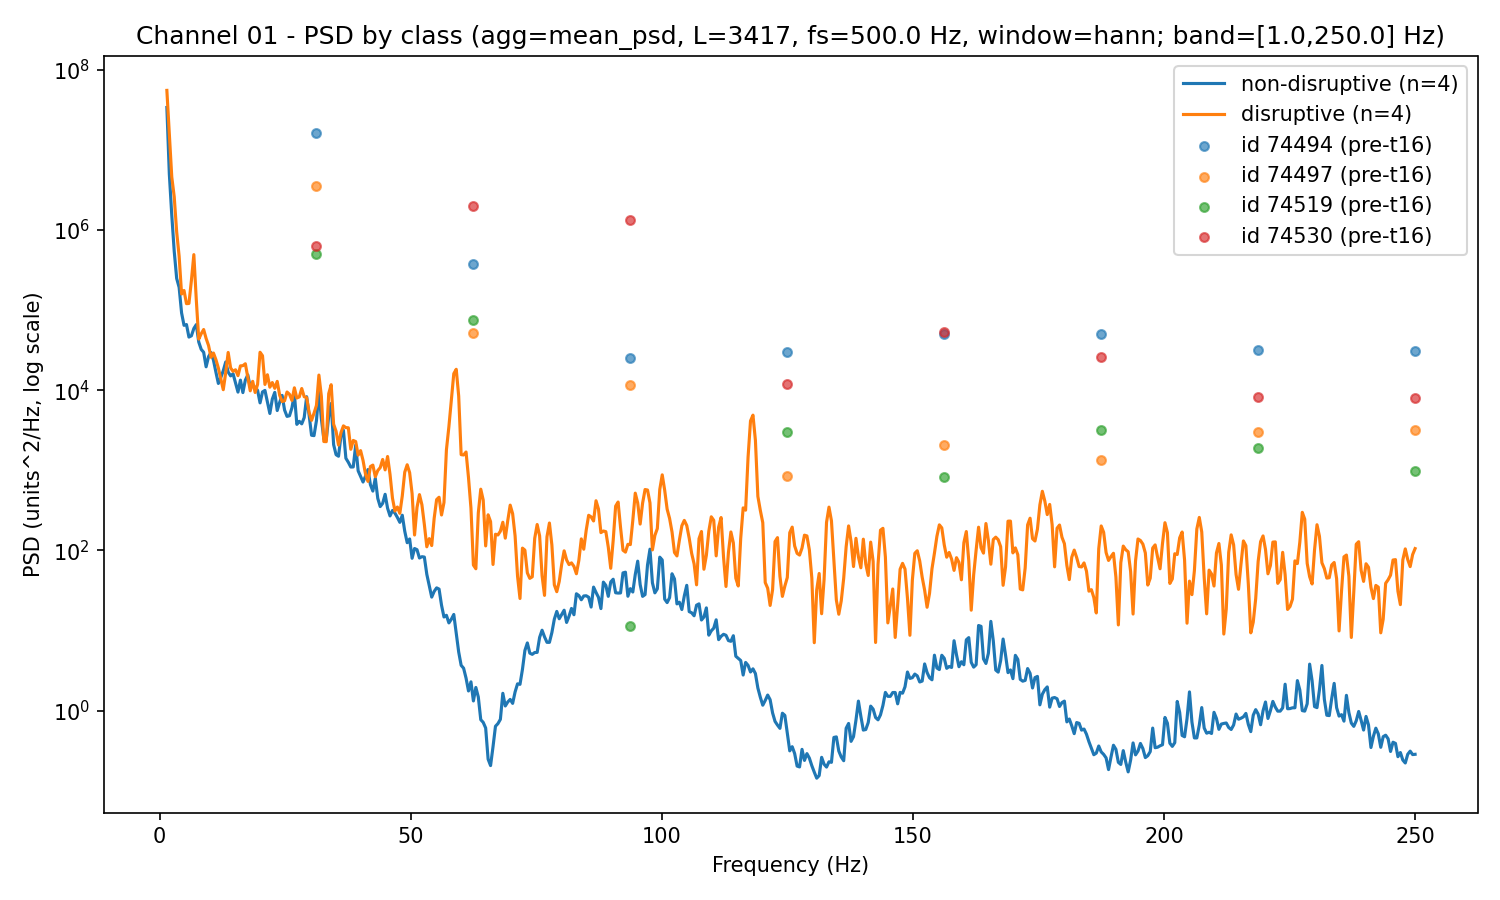
\includegraphics[width=.8\linewidth]{psd/psd_channel_01_mean_psd_band_1_250.png}
    \caption{Plasma Current}
    \label{fig:psd_channel_01_mean_psd_band_1_250}
  \end{subfigure}
  \begin{subfigure}{.5\textwidth}
    \centering
    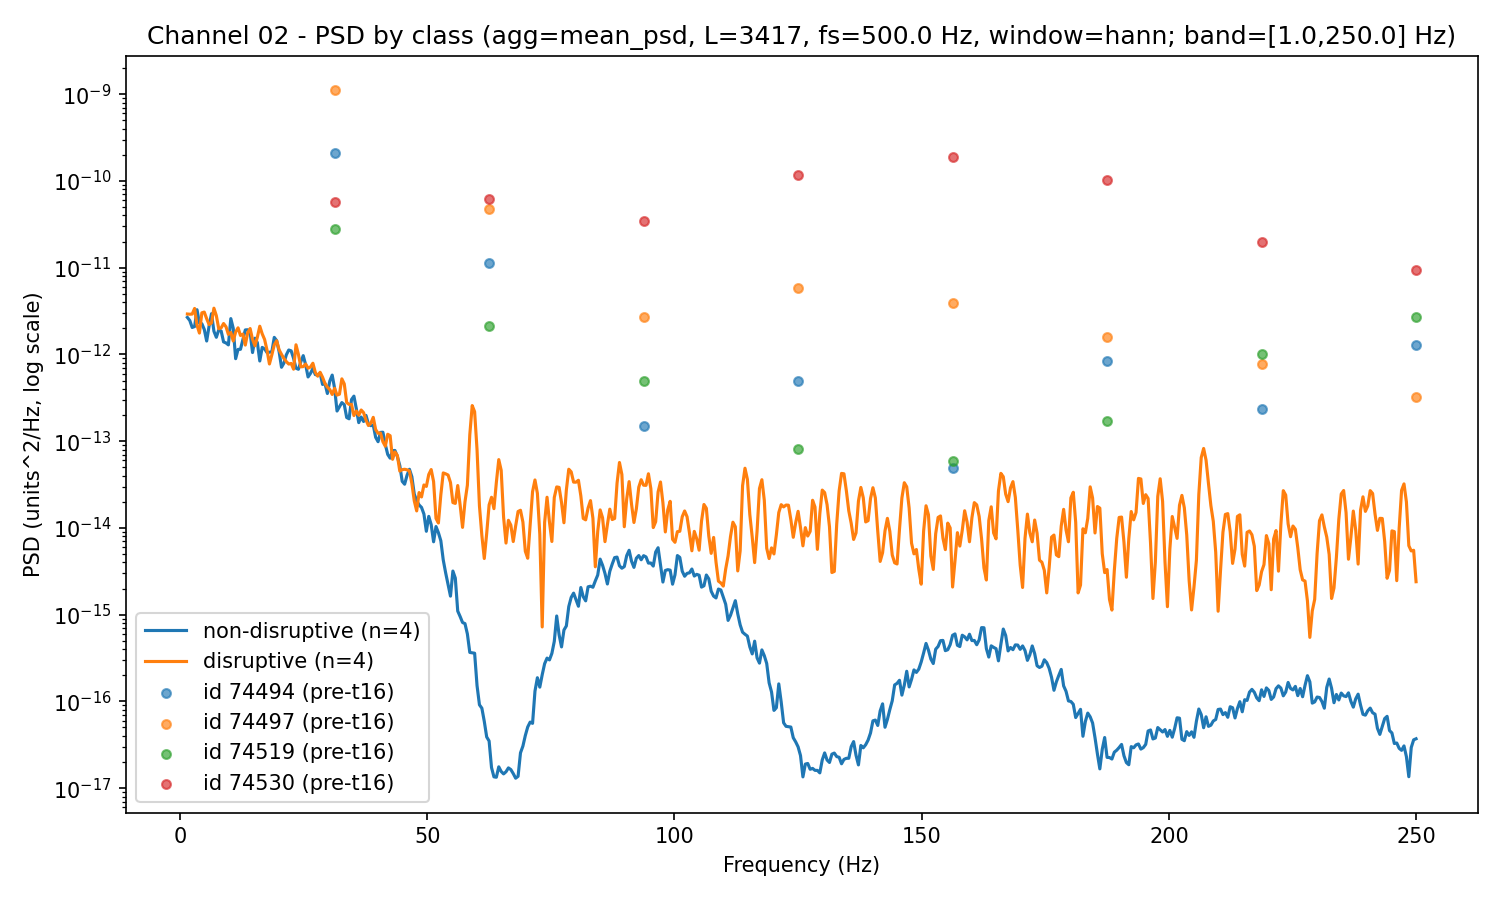
\includegraphics[width=.8\linewidth]{psd/psd_channel_02_mean_psd_band_1_250.png}
    \caption{Mode Lock Amplitude}
    \label{fig:psd_channel_02_mean_psd_band_1_250}
  \end{subfigure}
  \begin{subfigure}{.5\textwidth}
    \centering
    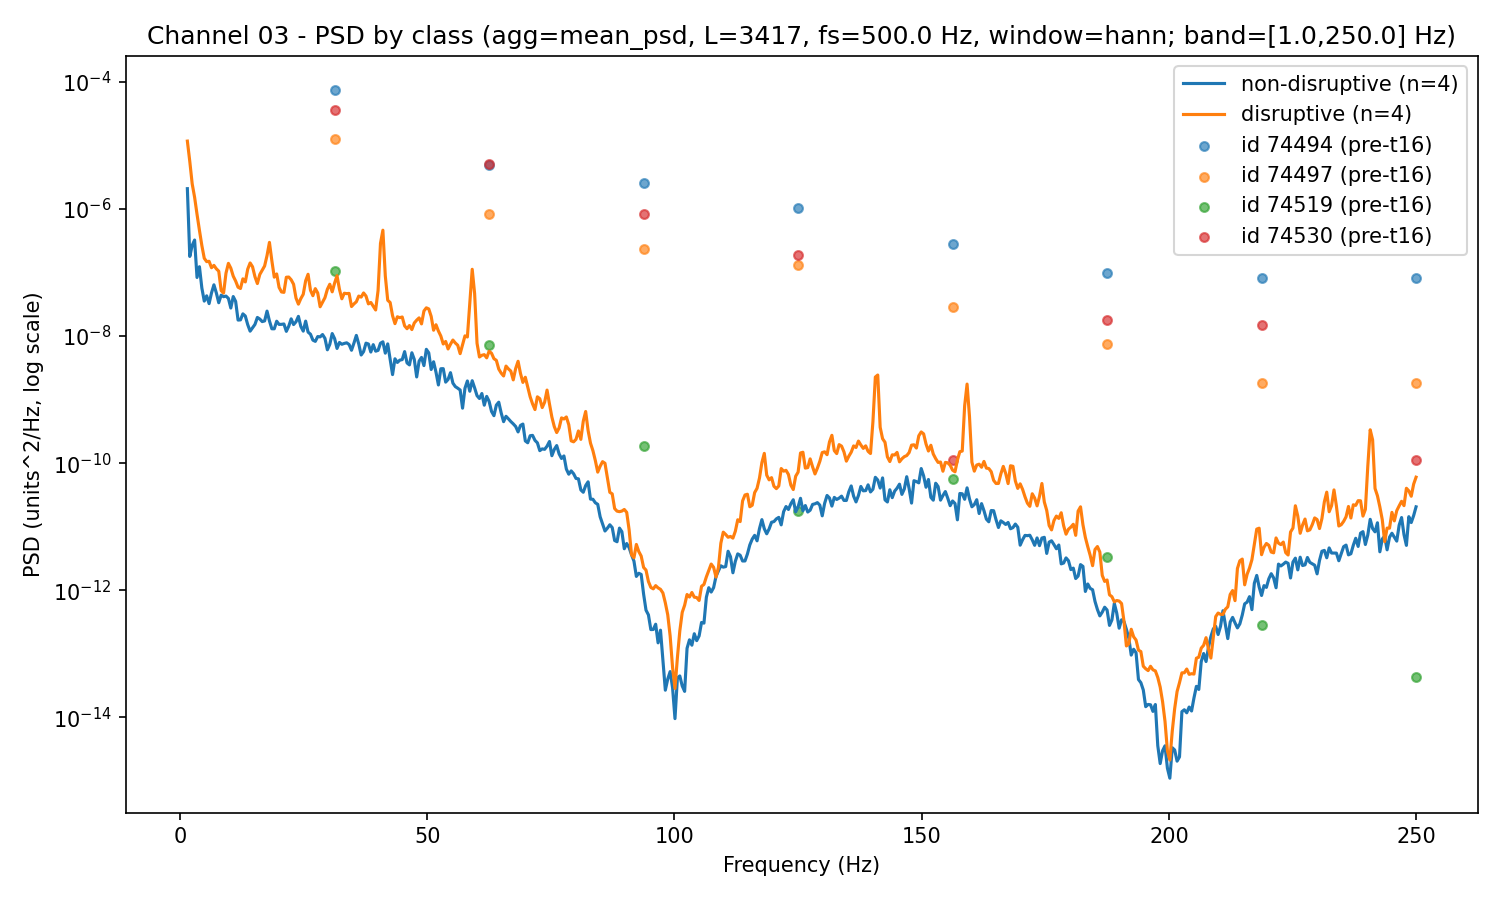
\includegraphics[width=.8\linewidth]{psd/psd_channel_03_mean_psd_band_1_250.png}
    \caption{Plasma internal inductance}
    \label{fig:psd_channel_03_mean_psd_band_1_250}
  \end{subfigure}
  \begin{subfigure}{.5\textwidth}
    \centering
    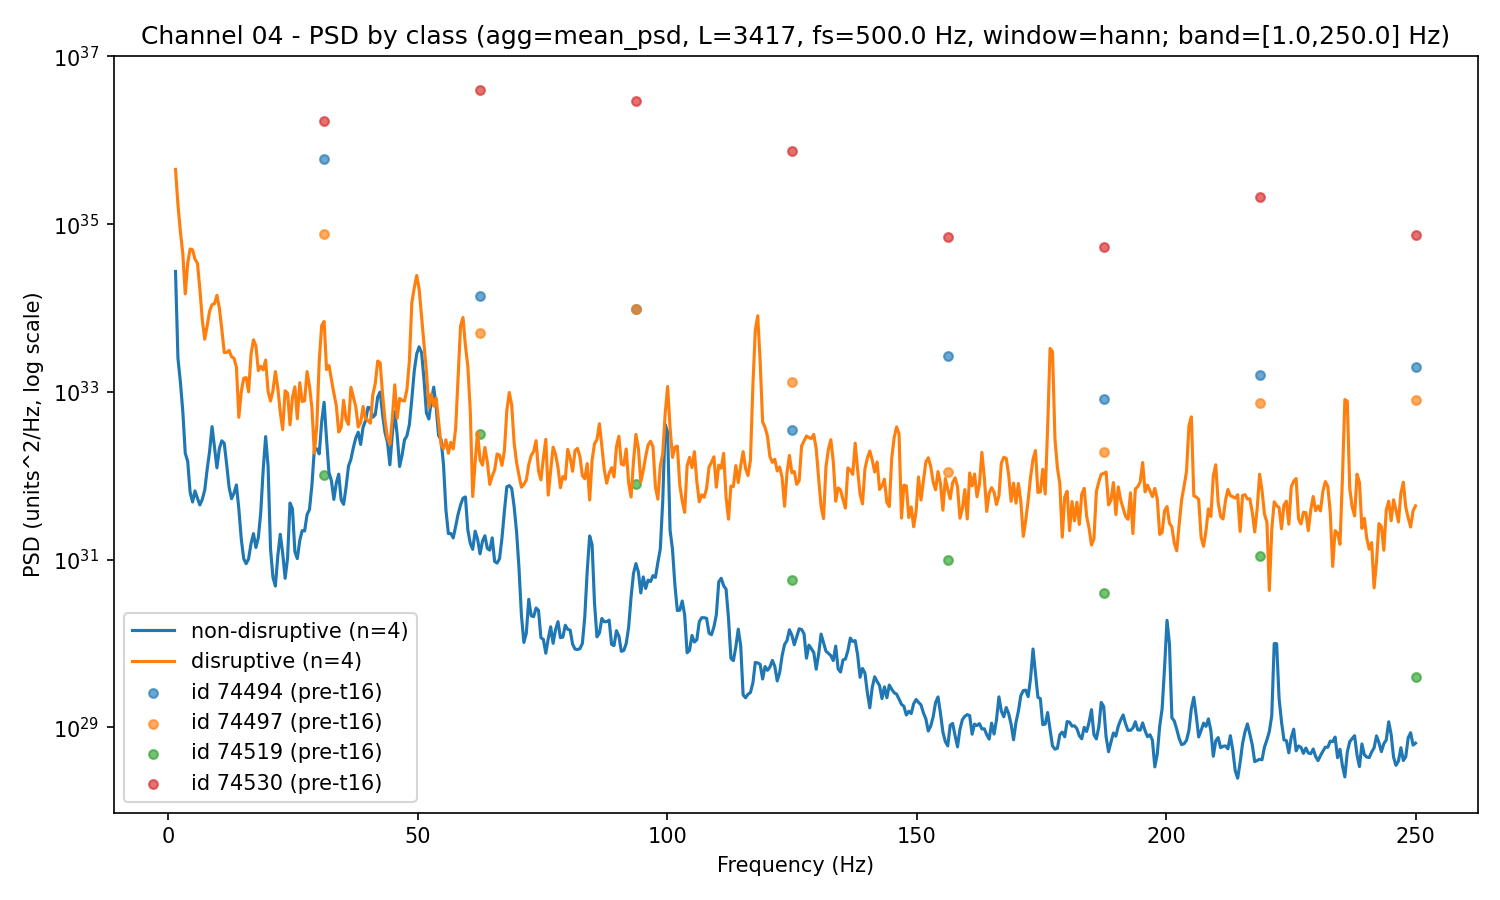
\includegraphics[width=.8\linewidth]{psd/psd_channel_04_mean_psd_band_1_250.png}
    \caption{Plasma density}
    \label{fig:psd_channel_04_mean_psd_band_1_250}
  \end{subfigure}
  \begin{subfigure}{.5\textwidth}
    \centering
    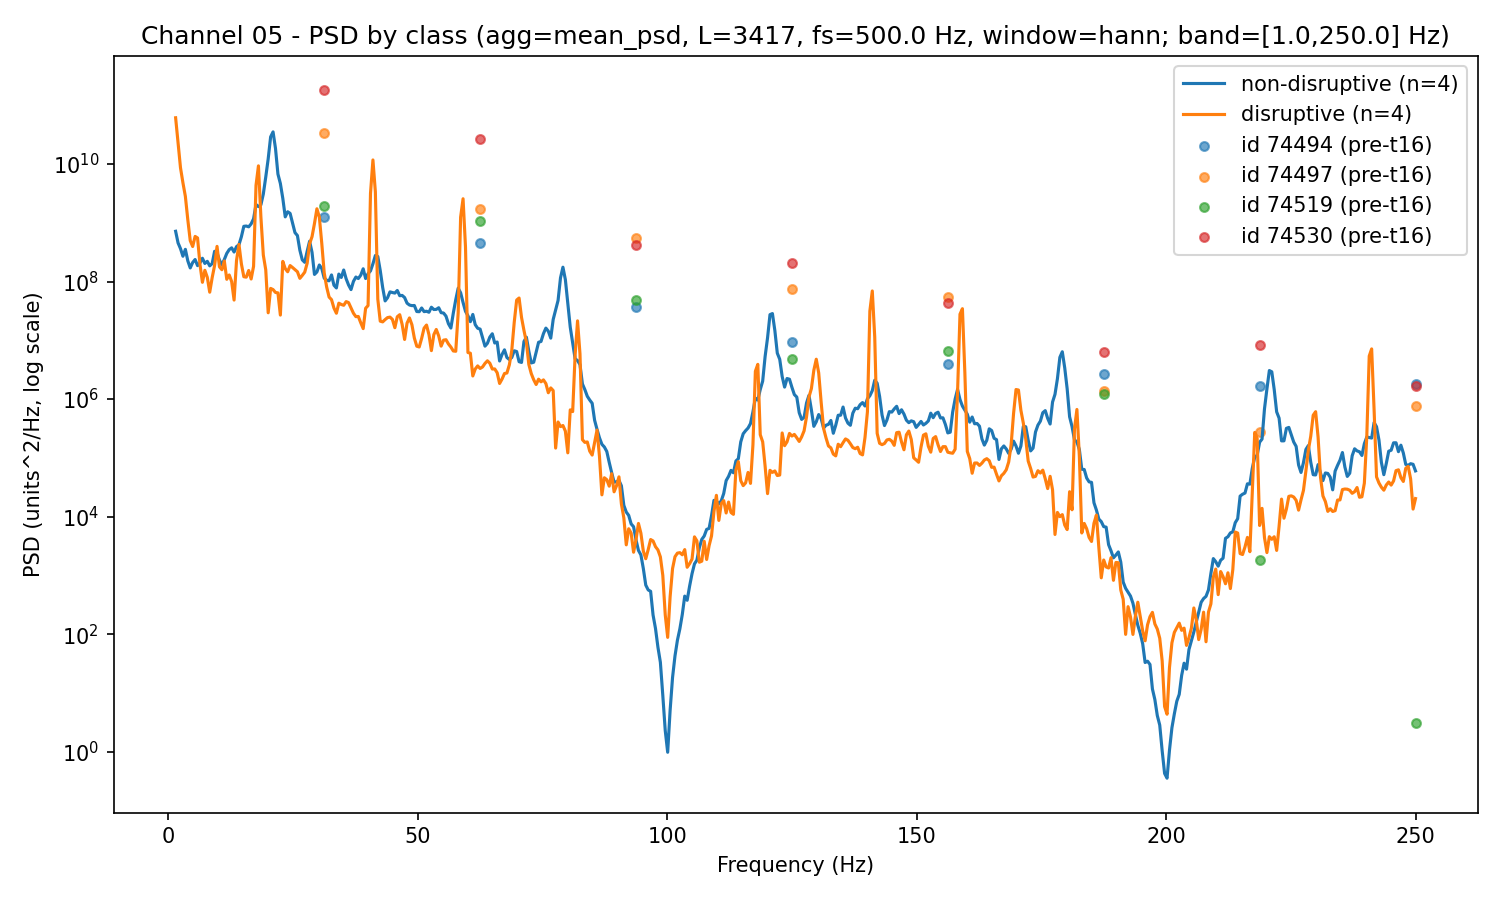
\includegraphics[width=.8\linewidth]{psd/psd_channel_05_mean_psd_band_1_250.png}
    \caption{Stored diamagnetic energy time derivative}
    \label{fig:psd_channel_05_mean_psd_band_1_250}
  \end{subfigure}
  \begin{subfigure}{.5\textwidth}
    \centering
    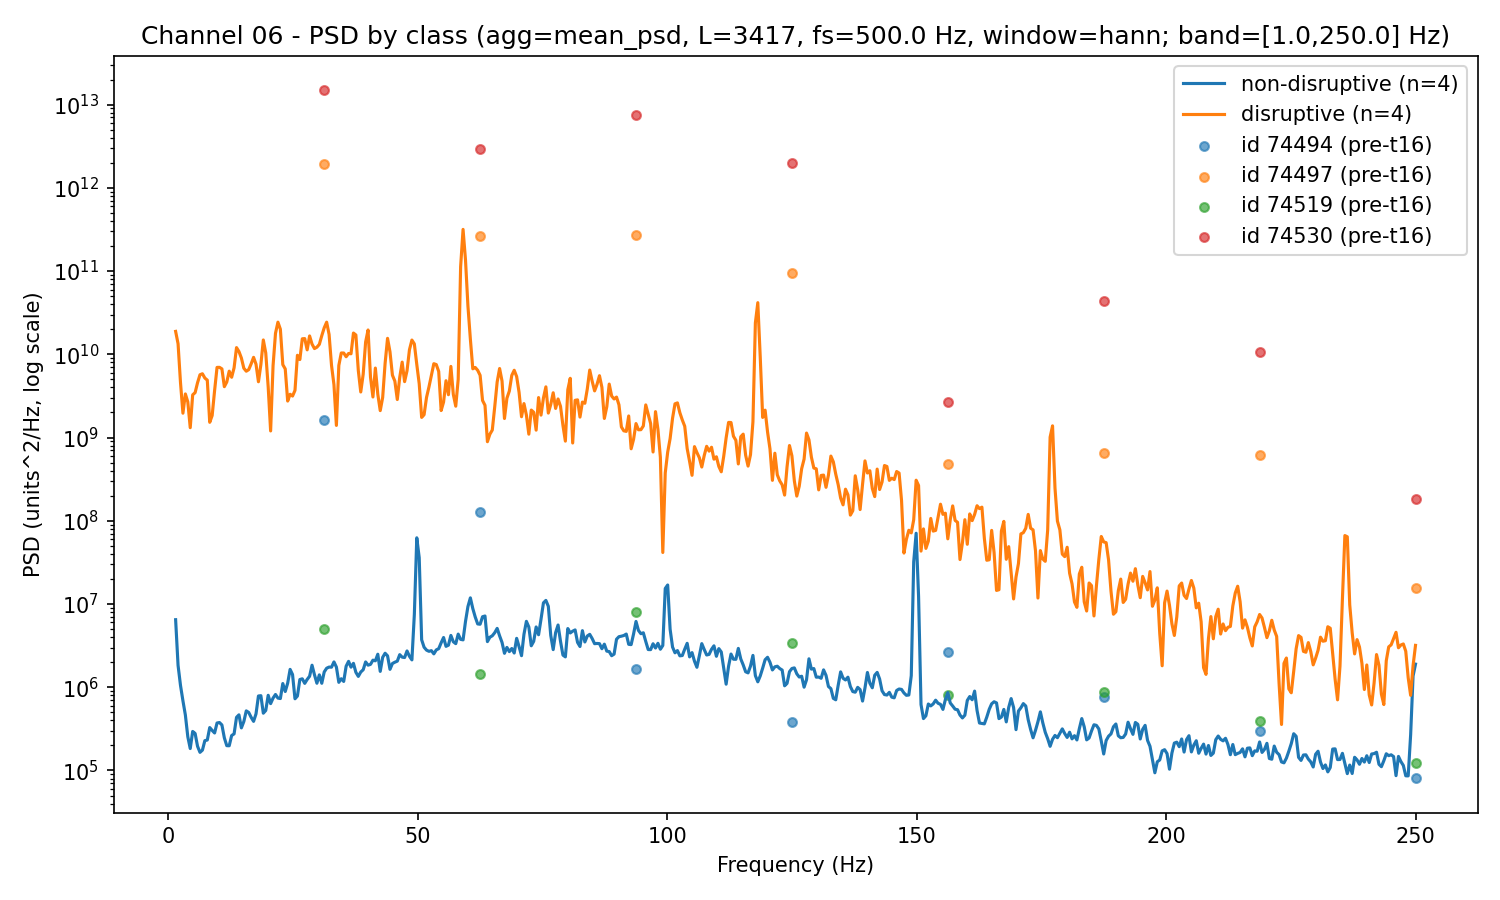
\includegraphics[width=.8\linewidth]{psd/psd_channel_06_mean_psd_band_1_250.png}
    \caption{Radiated Power}
    \label{fig:psd_channel_06_mean_psd_band_1_250}
  \end{subfigure}
  \begin{subfigure}{\textwidth}
    \centering
    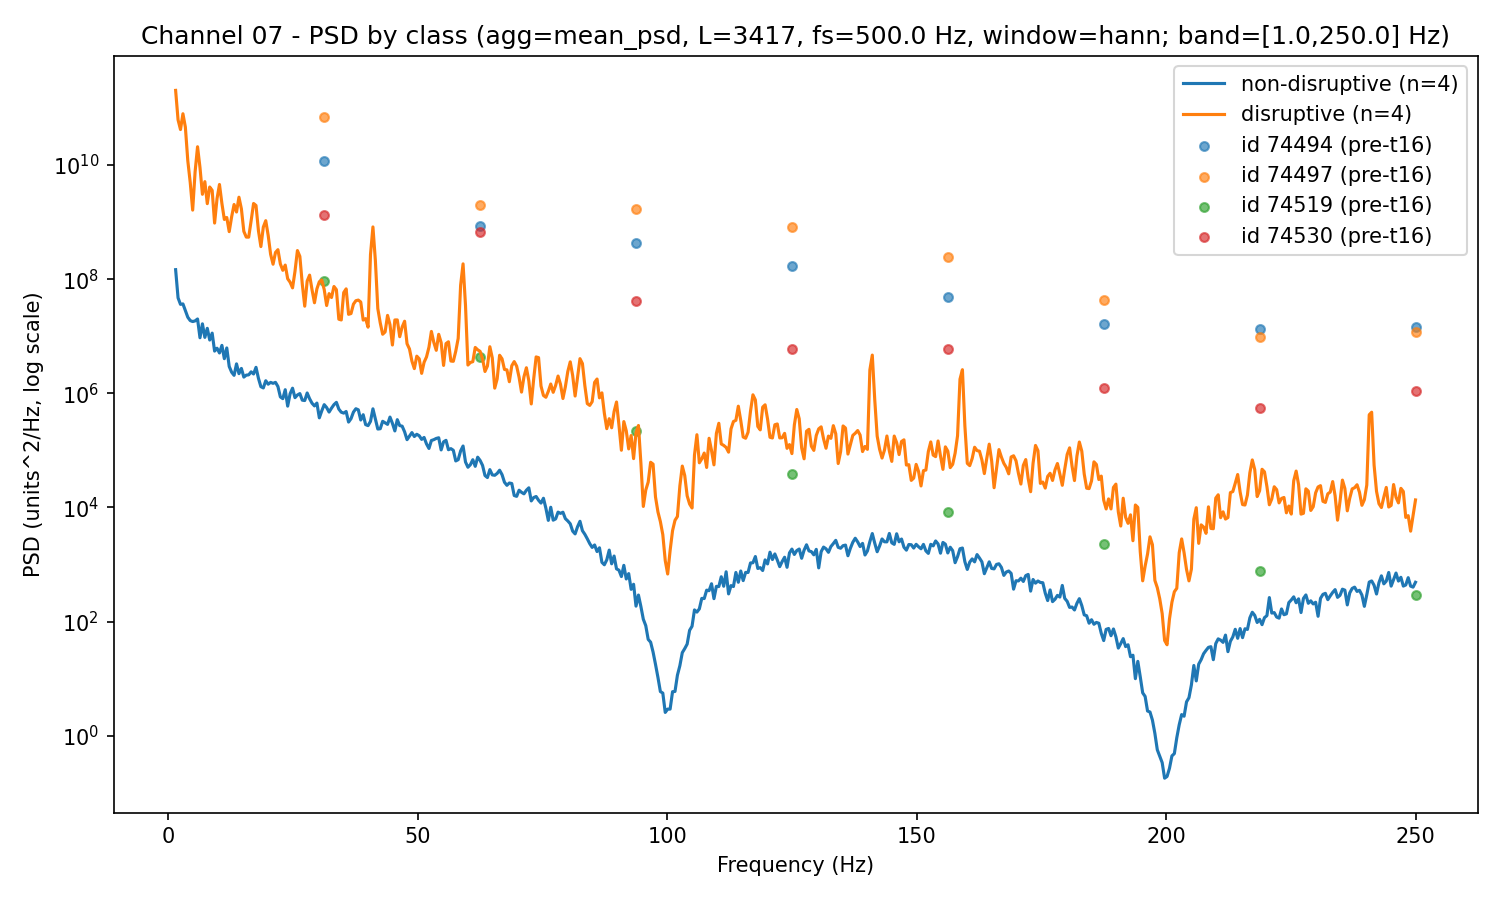
\includegraphics[width=.6\linewidth]{psd/psd_channel_07_mean_psd_band_1_250.png}
    \caption{Total Input power}
    \label{fig:psd_channel_07_mean_psd_band_1_250}
  \end{subfigure}
  \caption{Power Spectral Density of the signals used in the \ac{APODIS} algorithm}
  \label{fig:psd}
\end{figure}

Even though, there are some limitations to this approach. First, a window-based approach does not take into account large temporal dependencies of the data. This means that the model may not be able to capture the dynamics of the plasma behavior over time. Second, \ac{SVM} models with non-linear kernels have a complexity between $O(n^2)$ and $O(n^3)$, where $n$ is the number of training samples. This means that the model may not be able to scale to large datasets \autocite{kekulawalaSupportVectorMachines2024}. Third, even though \ac{SVM} models do not require a balanced dataset, the model could be biased towards the majority class, leading to a high false negative rate \autocite{10.1007/978-3-540-30115-8_7}. This is particularly important in this project, as the number of non-disruptive discharges is much higher than the number of disruptive discharges, as shown in \autoref{tab:campaigns}.

\section{Alternative approaches}

This project aims to explore alternative approaches to anomaly detection in nuclear fusion, focusing on the use of other \ac{ML} algorithms. Models used in this project can be grouped into three categories: decision trees based models, machine vector support based models and deep learning models. For each category, there are two subcategories: outlier detection and binary classification. Outlier detection models are trained on a single class of data (non-disruptive discharges), and generate a decision boundary that separates the normal data from the anomalies. Supervised binary classification models are trained on both classes of data (disruptive and non-disruptive discharges), and generate a decision boundary that separates the two classes.

\subsection{Decision Trees based models}

Decision trees are a type of \ac{ML} algorithm that uses a tree-like structure to make decisions based on the input data. This structure is built at the training phase, where the algorithm recursively splits the data into subsets based on the features that provide the most information gain. The resulting tree can be used to classify new data points by following the branches of the tree based on their feature values \autocite{1522531}.

\subsubsection{Outlier detection}

Decision trees can be used for outlier detection by training the model on a single class of data (non-disruptive discharges) and identifying instances that fall outside the normal patterns. The decision tree learns the characteristics of the normal data and can flag instances that do not conform to these patterns as potential anomalies. 

\ac{IForest} detects anomalies by explicitly isolating them through random binary partitioning, rather than estimating a density of normal data. Each \emph{isolation tree} is grown on a subsample of size $\psi$ by recursively selecting a feature uniformly at random and a split value uniformly within its observed range at the current node; growth stops when a point is isolated or a height limit is reached. The \emph{path length} $h(x)$ of an instance $x$ is the number of edges from the root to the external node where $x$ is separated. Anomalies, being few and different, tend to have shorter paths than regular points.\autocite{inproceedings}

To compare path lengths across different sample sizes, \textcite{inproceedings} normalize by the expected path length of an unsuccessful search in a binary tree,
\begin{equation}
c(n)\;=\;2\,H(n-1)\;-\;\frac{2(n-1)}{n},
\qquad
H(m)=\sum_{k=1}^{m}\frac{1}{k}\approx \ln(m)+\gamma,
\label{eq:expected-path-length}
\end{equation}
and define the ensemble anomaly score for subsample size $\psi$ as
\begin{equation}
s(x,\psi)\;=\;2^{-\; \mathbb{E}[\,h(x)\,]/c(\psi)}.
\label{eq:isolation-forest-score}
\end{equation}
Scores $s(x)\approx 1$ indicate strong anomalies ($h(x)\ll c(\psi)$), whereas $s(x)\approx 0.5$ is characteristic of inliers. With $t$ trees and subsample size $\psi$, training and scoring run in $\mathcal{O}\big(t\,\psi\log\psi\big)$ time and require $\mathcal{O}(t\,\psi)$ memory, which makes the method suitable for high-volume tabular data.\autocite{inproceedings}

\emph{\ac{EIF}} replaces axis-aligned splits by randomly oriented hyperplanes (or, equivalently, applies random rotations per tree), improving rotational invariance and reducing scoring artifacts near oblique boundaries without materially increasing computational cost.\autocite{haririExtendedIsolationForest2019}

\subsubsection{Binary classification}

If labelled data of both classes exist, standard decision-tree classifiers or ensembles (Random Forests, Gradient Boosting) can draw an explicit boundary between them. With sufficient minority class samples, these models usually outperform outlier detection models, as the tree learns exactly which feature ranges characterize each class rather than inferring a boundary from a single class. In practice, binary trees are common in fraud detection and network-intrusion datasets, where even a modest number of confirmed attack records allows the model to reach high recall without over-flagging harmless traffic \autocite{354051491,binary-classification-for-fraud-detection}.

For this project, a \ac{GBDT} classifier with a logistic objective is employed. The ensemble produces an additive margin
\[
F(x)=\sum_{t=1}^{T} f_t(x),
\]
which is mapped to a sigmoidal score
\begin{equation}
p(x)=\sigma\big(F(x)\big)=\frac{1}{1+e^{-F(x)}}.
\label{eq:gbdt-sigmoid}
\end{equation}
The regularized training objective is
\begin{equation}
\mathcal{L}(\{f_t\}) \;=\; \sum_{i=1}^{N} w_i\,\ell\!\left(y_i,\,F(x_i)\right) \;+\; \sum_{t=1}^{T} \Omega\!\left(f_t\right),
\label{eq:gbdt-objective}
\end{equation}
where \(y_i\in\{0,1\}\) are labels, \(w_i>0\) are sample or class weights, \(\Omega(\cdot)\) penalizes tree complexity (e.g., number of leaves and \(L_2\) regularization of leaf values), and \(\ell\) is the logistic loss

\begin{equation}
\ell(y,F) \;=\; -\,y\,\log \sigma(F)\;-\;(1-y)\,\log\bigl(1-\sigma(F)\bigr).
\label{eq:logistic-loss}
\end{equation}

At each boosting iteration the new tree \(f_t\) is fitted to (an approximation of) the negative gradient of the loss with respect to \(F\), typically using a second-order Taylor expansion to score candidate splits.

The model outputs \(p(x)\in[0,1]\), a monotone transformation of the margin \(F(x)\). Under class or sample reweighting (\(w_i\neq 1\)), \(p(x)\) should be interpreted as a sigmoidal score rather than a calibrated posterior probability; the operating point is therefore chosen on a held-out temporal validation set by selecting a decision threshold \(\tau\) for \(\hat{y}(x)=\mathbb{1}[p(x)\ge\tau]\) that optimizes the task metric \autocite{friedmanGreedyFunctionApproximation2000,chenXGBoostScalableTree2016}.


\subsection{Support Vector Machine-based models}\label{sec:svm}

Support Vector Machines construct a maximum-margin separating surface in a (possibly) high-dimensional feature space, obtained via a mapping $\phi:\mathcal{X}\to\mathcal{H}$. In the linearly separable (hard-margin) case, the primal problem reads
\begin{equation}
\min_{w,b}\;\tfrac12\lVert w\rVert^2
\quad\text{s.t.}\quad
y_i\bigl(\langle w,\phi(x_i)\rangle + b\bigr)\;\ge\;1,\;\; i=1,\dots,N.
\label{eq:svm-hard-margin}
\end{equation}
For nonseparable data, slack variables $\xi_i\ge 0$ yield the soft-margin formulation
\begin{equation}
\begin{aligned}
\min_{w,b,\xi}\;\tfrac12\lVert w\rVert^2 + C\sum_{i=1}^N\xi_i
\quad\text{s.t.}\quad
y_i\bigl(\langle w,\phi(x_i)\rangle + b\bigr)\;\ge\;1-\xi_i,\;\; i=1,\dots,N,
\end{aligned}
\label{eq:svm-soft-margin}
\end{equation}
which is equivalent to minimizing the regularized empirical hinge loss
\begin{equation}
\min_{w,b}\;\; \lambda \lVert w\rVert^2 + \sum_{i=1}^N \max\bigl(0,\,1 - y_i(\langle w,\phi(x_i)\rangle+b)\bigr),
\quad \lambda=\tfrac{1}{2C}.
\label{eq:svm-empirical-hinge}
\end{equation}
Introducing Lagrange multipliers $\alpha_i\in[0,C]$ leads to the dual problem
\begin{equation}
\max_{\alpha}\;\sum_{i=1}^N \alpha_i \;-\; \tfrac12\sum_{i,j=1}^N \alpha_i\alpha_j y_i y_j \,K(x_i,x_j)
\quad\text{s.t.}\quad \sum_{i=1}^N \alpha_i y_i = 0,
\label{eq:svm-dual}
\end{equation}
with kernel $K(x,x')=\langle \phi(x),\phi(x')\rangle$. Only training points with $\alpha_i>0$ (the \emph{support vectors}) contribute to the decision function
\begin{equation}
f(x) \;=\; \sum_{i=1}^N \alpha_i y_i K(x_i,x) + b,\qquad \hat{y}(x) = \mathrm{sign}\bigl(f(x)\bigr).
\label{eq:svm-decision-function}
\end{equation}
Typical kernels include the linear kernel, the polynomial kernel $K(x,x')={(\langle x,x'\rangle + c)}^d$, and the Gaussian RBF kernel $K(x,x')=\exp(-\gamma\lVert x-x'\rVert^2)$, which implicitly realize large (even infinite)-dimensional feature mappings without explicit construction of $\phi$ (the ``kernel trick'').

Class imbalance is handled by assigning different misclassification costs to the two classes, for example, $C_+$ and $C_-$ in the soft-margin constraints, or by per-sample weights in the primal/dual; this shifts the optimal margin to reflect asymmetric penalties and changes the operating point of the classifier. The raw SVM output $f(x)$ is a signed margin rather than a calibrated posterior probability; if probabilistic scores are required, a monotone post-hoc calibration such as Platt scaling or isotonic regression can be fitted on held-out data.

SVM training solves a convex quadratic program; modern implementations exploit decomposition or SMO-type methods for scalability, and linear SVM solvers are preferred in very high-dimensional sparse settings \autocite{cortesSupportvectorNetworks1995b,scholkopfLearningKernelsSupport2001}. Because of the high complexity of the dual problem, \ac{SVM}s are not suitable for very large datasets, and their training time scales with the square of the number of samples. However, they are effective in high-dimensional spaces and can handle non-linear decision boundaries through kernelization.

\subsubsection{Convolutional Neural Networks}\label{sec:cnn}

\ac{CNN} are deep architectures that learn local filters shared across time, forming hierarchical feature extractors well suited to multichannel tokamak diagnostics. Their key inductive bias is translation equivariance: a precursor with the same local morphology is detected regardless of its absolute time within a discharge, which is desirable for early identification of \ac{MHD} activity.

Consider a window $x \in \mathbb{R}^{C \times T}$ of $C$ synchronized signals and $T$ samples. A bank of $M$ one-dimensional filters $K \in \mathbb{R}^{M \times C \times L}$ with optional dilation $d \in \mathbb{N}$ produces
\begin{equation}
z_{m}[t] \;=\; \sum_{c=1}^{C}\sum_{\ell=0}^{L-1} K_{m,c,\ell}\; x_{c}[\,t + d\,\ell\,] \;+\; b_{m},
\qquad m=1,\dots,M,
\label{eq:conv1d}
\end{equation}
followed by pointwise nonlinearities $y_m[t]=\phi(z_m[t])$. Denoting the discrete shift operator $(\mathcal{T}_\Delta x)[t]=x[t-\Delta]$, a convolutional layer $\mathcal{F}$ satisfies
\begin{equation}
\mathcal{F}\!\big(\mathcal{T}_\Delta x\big)\;=\;\mathcal{T}_\Delta\!\big(\mathcal{F}(x)\big),
\label{eq:equivariance}
\end{equation}
which explains why shared local kernels are effective to detect precursors irrespective of their position in time. Stacking layers, and optionally using dilation, enlarges the effective receptive field so that both short-lived bursts and longer build-ups can be represented within the same network depth.

When diagnostics are projected to the time-frequency plane, e.g.\ through the short-time Fourier transform (\ac{STFT}),
\begin{equation}
X(\tau,\omega)\;=\;\int_{-\infty}^{\infty} x(t)\, w(t-\tau)\, e^{-\,\mathrm{i}\,\omega t}\,\mathrm{d}t,
\label{eq:stft}
\end{equation}
the magnitude (often log-magnitude) spectrogram $|X(\tau,\omega)|$ becomes a two-dimensional tensor. In this representation, early \ac{MHD} activity tends to manifest as band-localized energy growth and evolving inter-band couplings; two-dimensional \ac{CNN}s learn filters that are selective to such patterns across frequency and time.

For binary detection, a \ac{CNN} outputs a probability $p\in(0,1)$ for a window to be disruptive. Class imbalance can be addressed during training with a weighted cross-entropy,
\begin{equation}
\mathcal{L}\;=\;-\frac{1}{N}\sum_{n=1}^{N}\Big[\,w_1\, y_n\log p_n \;+\; w_0\,(1-y_n)\log(1-p_n)\,\Big],
\label{eq:weighted_bce}
\end{equation}
where $y_n\in\{0,1\}$ are labels, $p_n$ the predicted probabilities, and $w_1,w_0>0$ the class weights. This objective couples naturally with convolutional feature extractors in either the time domain (Eq.~\eqref{eq:conv1d}) or the time-frequency domain (Eq.~\eqref{eq:stft}).

Empirically, \ac{CNN}-based predictors have demonstrated accurate and low-latency disruption detection on \ac{JET} using spatiotemporal profiles and spectrograms, and on \ac{EAST} using fully convolutional models over raw multichannel time series, without the need for hand-crafted features \cite{aymerichCNNDisruptionPredictor2023,guoDisruptionPredictionUsing2020}.
